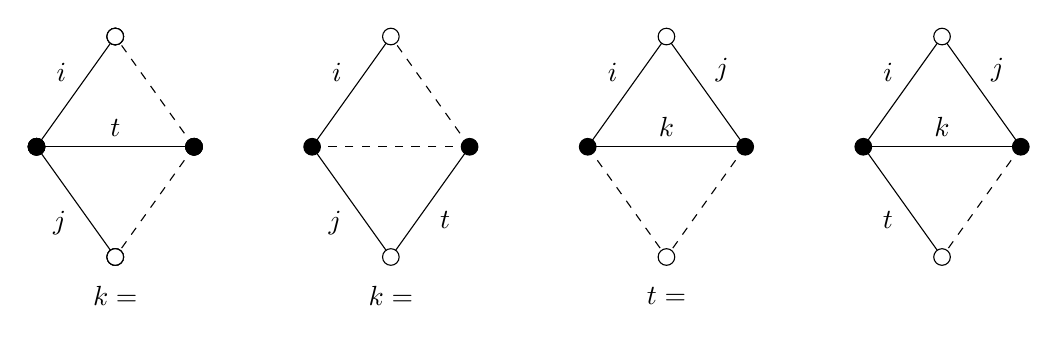
\begin{tikzpicture}
	\def\c{1.4}
	\def\d{0.5}
	\coordinate (a1) at (1,0);
	\coordinate (a2) at (0,\c);
	\coordinate (a3) at (-1,0);
	\coordinate (a4) at (0,-\c);
	\draw (a2) -- (a3) node[midway,above left] {$i$};
	\draw (a3) -- (a4) node[midway,below left] {$j$};
	\draw (a1) -- (a3) node[midway,above] {$t$};
	\draw[dashed] (a1) -- (a2);
	\draw[dashed] (a1) -- (a4);
	\draw[fill=white] (a2) circle (3pt);
	\draw[fill=white] (a4) circle (3pt);
	\draw[fill=black] (a1) circle (3pt);
	\draw[fill=black] (a3) circle (3pt);
	\node at (0,-\c-\d) {$k=\eh$};
	
	\def\a{3.5}
	\coordinate (b1) at (\a+1,0);
	\coordinate (b2) at (\a,\c);
	\coordinate (b3) at (\a-1,0);
	\coordinate (b4) at (\a,-\c);
	\draw (b2) -- (b3) node[midway,above left] {$i$};
	\draw (b3) -- (b4) node[midway,below left] {$j$};
	\draw (b1) -- (b4) node[midway,below right] {$t$};
	\draw[dashed] (b1) -- (b2);
	\draw[dashed] (b1) -- (b3);
	\draw[fill=white] (a2) circle (3pt);
	\draw[fill=white] (a4) circle (3pt);
	\draw[fill=black] (a1) circle (3pt);
	\draw[fill=black] (a3) circle (3pt);
	\draw[fill=white] (b2) circle (3pt);
	\draw[fill=white] (b4) circle (3pt);
	\draw[fill=black] (b1) circle (3pt);
	\draw[fill=black] (b3) circle (3pt);
	\node at (\a,-\c-\d) {$k=\eh$};
	
	\coordinate (c1) at (2*\a+1,0);
	\coordinate (c2) at (2*\a,\c);
	\coordinate (c3) at (2*\a-1,0);
	\coordinate (c4) at (2*\a,-\c);
	\draw (c2) -- (c3) node[midway,above left] {$i$};
	\draw (c1) -- (c2) node[midway,above right] {$j$};
	\draw (c1) -- (c3) node[midway,above] {$k$};
	\draw[dashed] (c3) -- (c4);
	\draw[dashed] (c1) -- (c4);
	\draw[fill=white] (a2) circle (3pt);
	\draw[fill=white] (a4) circle (3pt);
	\draw[fill=black] (a1) circle (3pt);
	\draw[fill=black] (a3) circle (3pt);
	\draw[fill=white] (c2) circle (3pt);
	\draw[fill=white] (c4) circle (3pt);
	\draw[fill=black] (c1) circle (3pt);
	\draw[fill=black] (c3) circle (3pt);
	\node at (2*\a,-\c-\d) {$t=\eh$};
	
	\coordinate (d1) at (3*\a+1,0);
	\coordinate (d2) at (3*\a,\c);
	\coordinate (d3) at (3*\a-1,0);
	\coordinate (d4) at (3*\a,-\c);
	\draw (d2) -- (d3) node[midway,above left] {$i$};
	\draw (d1) -- (d2) node[midway,above right] {$j$};
	\draw (d1) -- (d3) node[midway,above] {$k$};
	\draw (d3) -- (d4) node[midway,below left] {$t$};
	\draw[dashed] (d1) -- (d4);
	\draw[fill=white] (a2) circle (3pt);
	\draw[fill=white] (a4) circle (3pt);
	\draw[fill=black] (a1) circle (3pt);
	\draw[fill=black] (a3) circle (3pt);
	\draw[fill=white] (d2) circle (3pt);
	\draw[fill=white] (d4) circle (3pt);
	\draw[fill=black] (d1) circle (3pt);
	\draw[fill=black] (d3) circle (3pt);
	\end{tikzpicture}